\section{Bestrahlungsplanung}
\label{sec:Bestrahlungsplanung}
Das PTV ist bereits in den CT-Daten eingezeichnet und als nächstes wird die Fußkontur als Body-Struktur eingezeichnet.
Außerdem müssen Gegenstände, wie zum Beispiel Lagerungshilfen oder die Patientenliege, die sich im Strahlengang befinden
ebenfalls als Struktur eingezeichnet werden. Das Ziel der Bestrahlungsplanung ist, dass das PTV mit der
$\SI{95}{\percent}$-Isodosenlinie umgeschlossen wird.
Für die Bestrahlung des Fußes werden zwei Felder der Größe $\SI{15}{\centi\meter}$ x $\SI{15}{\centi\meter}$ erstellt,
welche eine Einstrahlungsrichtung von jeweils 0$^\circ$ und 180$^\circ$ besitzen.
Es werden $\SI{6}{\mega\volt}$ Photonen verwendet und der Bestrahlungsplan wird auf \enquote{$100\%$ target mean} normiert.
Außerdem werden die beiden Felder mit Hilfe von MLCs an die Struktur angepasst, sodass das umliegende Gewebe besser geschont werden kann.
Dazu werden die Lamellen des MLCs einzeln eingestellt.
Die Einstellung der MLCs der beiden Felder ist in Abbildung \ref{abb:MLC} dargestellt.

\begin{figure}[H]
  \centering
  \begin{subfigure}{\textwidth}
    \centering
    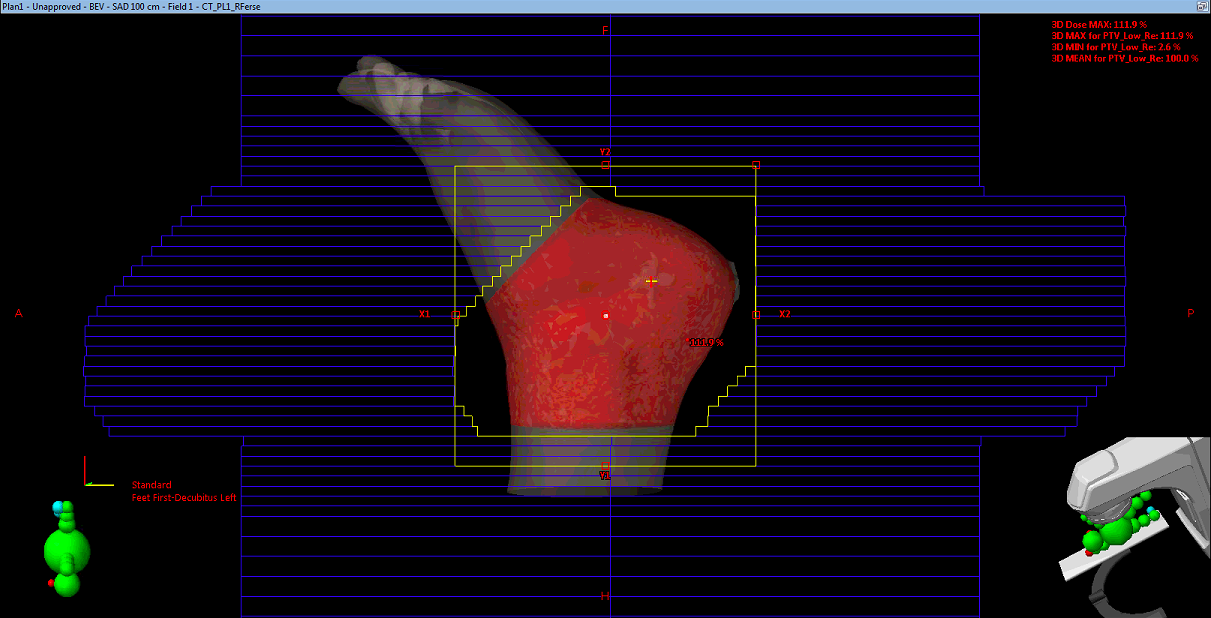
\includegraphics[height = 5cm]{Bilder/MLCFeld1.png}
    \caption{}
  \end{subfigure}
  \begin{subfigure}{\textwidth}
    \centering
    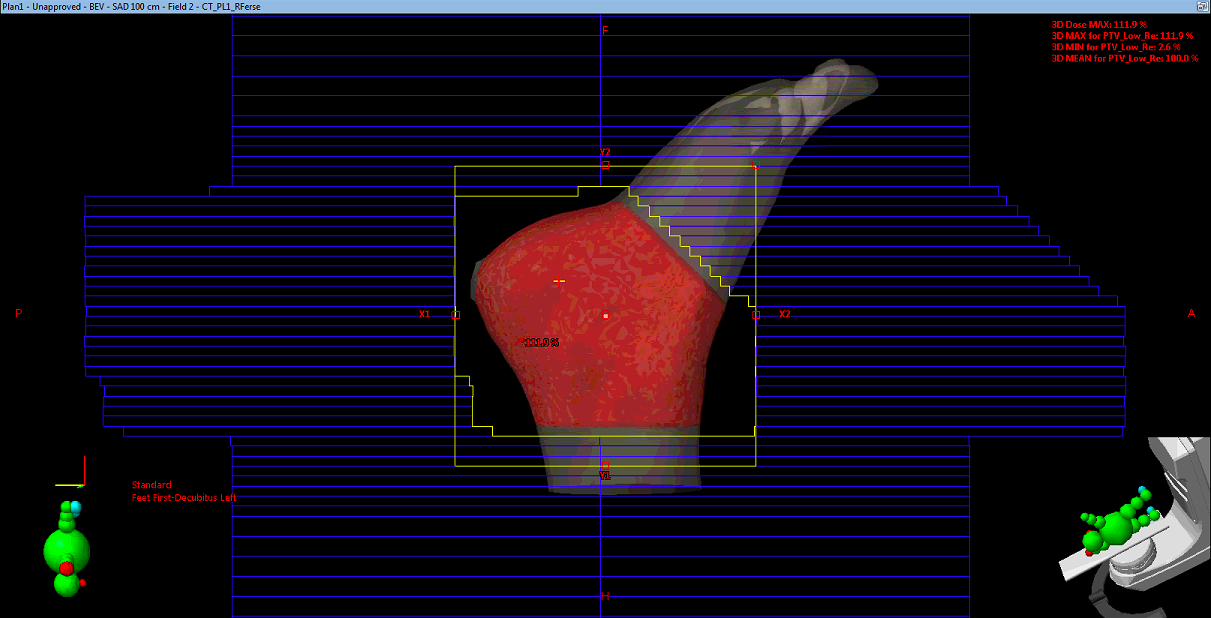
\includegraphics[height=5cm]{Bilder/MLCFeld2.png}
    \caption{}
  \end{subfigure}
  \caption{Darstellung der Lamellenpositionen der beiden Felder. Bei a) die Positionen bei dem Feld bei $0°$ und bei b) die Positionen bei dem Feld bei $180°$.}
  \label{abb:MLC}
\end{figure}
